\begin{enumerate}[label=\thesection.\arabic*.,ref=\thesection.\theenumi]
\numberwithin{equation}{enumi}

\item Question-The open loop transfer function of a unity feedback system is given by
\begin{align*}
 G(s)=\frac{\pi e^{-0.25s}}{s}
\end{align*}
\item Find  $\text{Re} \cbrak{G(\j \omega)}$ and  $\text{Im} \cbrak{G(\j \omega)}$
\newline
\solution 
substitute \begin{align}
S=j\omega
\end{align}
we get \begin{align}
G(j\omega)&=-\frac{\pi}{\omega}(\sin{0.25\omega}+j\cos{0.25\omega})
\end{align}
\begin{align}
 \text{Re} \cbrak{G(\j \omega)}=-\frac{\pi}{\omega}(\sin{0.25\omega}) 
\end{align}
\begin{align}
 \text{Im} \cbrak{G(\j \omega)}=-\frac{\pi}{\omega}(j\cos{0.25\omega}) 
\end{align}
\item Sketch the Nyquist plot.
\\
\solution The Nyquist plot is a graph of $\text{Re} \cbrak{G(\j \omega)}$  vs $\text{Im} \cbrak{G(\j \omega)}$.
The following python code generates the Nyquist plot in Fig.  \ref{fig:ee18btech11007}
\begin{lstlisting}
codes/ee18btech11007/nyquist.py
\end{lstlisting}
%
\begin{figure}[!h]
  \includegraphics[width=\columnwidth]{./figs/ee18btech11007.eps}
  \caption{}
  \label{fig:ee18btech11007}
\end{figure}
%
\item Find the point at which the Nyquist plot of G(s) passes through negative real axis
\newline
\solution
\begin{align}
G(s)=\frac{\pi e^{-0.25s}}{s}
\end{align}

 Nyquist plot cuts the negative real
Axis at $\omega$ = phase cross over frequency,at phase cross over frequency the phase of nyquist plot becomes -$\pi$ radians.
\
\newline substitute \begin{align}
s=j\omega.\end{align} 
\begin{align}
G(j\omega)&= -\frac{\pi}{\omega}(\sin{0.25\omega}+j\cos{0.25\omega})
\end{align}
\begin{align}
\angle G(j\omega)=-\pi/2 -0.25\omega.
\end{align}
\begin{align}
\angle G(j\omega)|_{\omega=\omega_{pc}}=-\pi
\end{align}
by solving for $\omega$ we get $\omega_{pc}=2\pi$.
\
\newline magnitude at any point is\begin{align}
X=|G(j\omega)|=\frac{\pi}{\omega}.    
\end{align} 
\
\newline substituting $\omega=2\pi$ in magnitude equation we get X=0.5.
\\
\newline so it intersects at (-0.5,0j)
\\
\newline we can verify with the following plot that it intersects at (-0.5,0j)

\\
\item Use Nyquist stability criterion to determine if the system is stable?
\newline
\solution
 \textbf{Nyquist Stability Criterion} - for  the stability of a closed loop transfer function G(s)/(1+G(s)*H(s)) ,the number of poles of G(s)*H(s) on right half of s-plane must equal the number of encirclement of nyquist contour of  G(s)*H(s) about the critical point -1+0j
\\
\newline we must find
\begin{align}
Z=P+N    
\end{align}
\
\begin{tabular}{ |p{4cm}||p{4cm}|  }
 \hline
 
 \hline
 Variable&Description\\
 \hline
 Z&no of poles of G(s)/(1+G(s)*H(s)) in the right half of s-plane\\
 \hline
 P&no of poles of G(s)*H(s) in right half of s-plane \\
 \hline
 N&no of encirclement of G(s)*H(s) about -1+j0 in clockwise direction\\
 
 \hline
\end{tabular}
\\
\newline NOTE-
\begin{itemize}
\item If a clockwise contour does not encircle zeros nor poles, then the plot will not encircle the origin.
\item If a clockwise contour encircles a zero, then the plot will encircle the origin clockwise once.
\item If a clockwise contour encircles a pole, then the plot will encircle the origin counterclockwise once.
\end{itemize}
\\
\newline from plot we get N=0 because there are no encirclements about -1+0j,and we already know P=0 since our G(s) doesnt have any poles on right half of s-plane
\begin{align}
Z=0+0=0
\end{align}
$\therefore$ the system is stable.



\end{enumerate}
